%% This skeleton file requires IEEEtran.cls version 1.6 or later.
%%
\documentclass[conference,letterpaper]{IEEEtran}
% If the IEEEtran.cls has not been installed into the LaTeX system files,
% manually specify the path to it:
% \documentclass[conference]{../sty/IEEEtran}
\IEEEoverridecommandlockouts
\overrideIEEEmargins

% some very useful LaTeX packages include:

%\usepackage{cite}      % Written by Donald Arseneau
                        % V1.6 and later of IEEEtran pre-defines the format
                        % of the cite.sty package \cite{} output to follow
                        % that of IEEE. Loading the cite package will
                        % result in citation numbers being automatically
                        % sorted and properly "ranged". i.e.,
                        % [1], [9], [2], [7], [5], [6]
                        % (without using cite.sty)
                        % will become:
                        % [1], [2], [5]--[7], [9] (using cite.sty)
                        % cite.sty's \cite will automatically add leading
                        % space, if needed. Use cite.sty's noadjust option
                        % (cite.sty V3.8 and later) if you want to turn this
                        % off. cite.sty is already installed on most LaTeX
                        % systems. The latest version can be obtained at:
                        % http://www.ctan.org/tex-archive/macros/latex/contrib/supported/cite/

\usepackage[pdftex]{graphicx}  % Written by David Carlisle and Sebastian Rahtz
                        % Required if you want graphics, photos, etc.
                        % graphicx.sty is already installed on most LaTeX
                        % systems. The latest version and documentation can
                        % be obtained at:
                        % http://www.ctan.org/tex-archive/macros/latex/required/graphics/
                        % Another good source of documentation is "Using
                        % Imported Graphics in LaTeX2e" by Keith Reckdahl
                        % which can be found as esplatex.ps and epslatex.pdf
                        % at: http://www.ctan.org/tex-archive/info/

%\usepackage{amsmath}   % From the American Mathematical Society
                        % A popular package that provides many helpful commands
                        % for dealing with mathematics. Note that the AMSmath
                        % package sets \interdisplaylinepenalty to 10000 thus
                        % preventing page breaks from occurring within multiline
                        % equations. Use:
\usepackage{multirow}
\usepackage{fixltx2e}
\usepackage{hyperref}
\usepackage[left=0.71in,top=0.94in,right=0.71in,bottom=1.18in]{geometry}
\setlength{\columnsep}{0.24in}
% correct bad hyphenation here
%\hyphenation{op-tical net-works semi-conduc-tor IEEEtran}


\begin{document}
% paper title
\title{\huge Social Network Analysis}

% author names and affiliations
\author{\authorblockN{Stefan Dimitrov}
\authorblockA{\textit{School of Computer Science}\\
\textit{McGill University}\\
\textit{Montreal, Quebec, Canada}\\
\textit{stefan.dimitrov@mail.mcgill.ca}\\}}

% make the title area
\maketitle
\begin{abstract}
This paper surveys a number of existing works on the topic of Social Network Analysis and presents some of the most essential concepts in the field. We focus on issues such as the definition of a Social Network and Social Network Analysis, important theories from sociology and psychology applicable to social networks in the digital age, the concept of influence and its importance for the analysis of social networks, and the buzzword technique known as Viral Marketing.
\\
\end{abstract}

% key words
\begin{keywords}
Social, network, influence, viral, marketing
\end{keywords}

\section{Introduction}
% no \PARstart
With the growing popularity of mobile devices and the omnipresence of high speed Internet connections, online social networks such as Twitter and Facebook have emerged to connect individuals and organizations.
Thus, it is of great interest to study the underlying theories which explain the formation, structure and functioning of social networks. Sociologists and psychologysts have made great progress in modeling human behaviour and relationships, 
the balance of power and influence in groups and the ideas powering viral information propagation in society. This paper aims to investigate the applicability of these existing theories to the recently emerged online social network services.
Gaining better understanding of the science behind these services will facilitate future work to solve important problems in social networks such as the identification of malicious or automated accounts publishing undesired commercial messages (SPAM) in social networks.\\
\indent
The following section presents an overview of existing works related to Social Network Analysis, which form the foundation for this paper. Later we define the most important concepts for the study of social networks, such as actors, relations and centrality.
Then we focus on influence in social networks and viral marketing. Finally, we conclude with a summary of our study.\\
%\hfill August 13, 2002

\section{Related work}
% no \PARstart
Weather has been linked with feature prices in the past, in particular with natural gas. The reason is because
natural gas is used for heating in the winter and for energy generation which powers air conditioning systems in the summer. 
Thus, short term temperature variations can cause volatility in the demand for natural gas. As Mu (2007) found, up to
50\% of the US demand for natural gas is affected by weather. [3] \\
\indent Furthermore, weather has been found to influence the intraday trading behaviour of traders by affecting their mood [4]. 
Chang et al. (2008) look into the overall stock market, but not gas equities in particular. \\
\indent I have not found any prior study attempting to predict the direction of daily returns for a gas equity based on
weather measurements and deviations from the mean temperature for a given day. While Mu (2007) looks into the effect of
weather shocks on gas features returns, he does not look into the psychological influence of weather variations on traders. \\


\section{Definition}

\begin{center}
\begin{figure}[hb]
\centering
%\includegraphics{imagen1.eps}
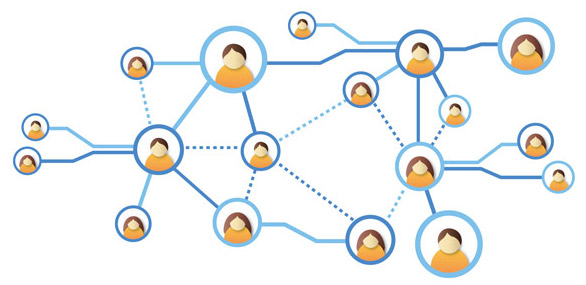
\includegraphics[width=3.2in]{social-network-grid}
\caption{
A graph of a social network. The thikness of lines represents the strength of relations between actors. [1]
}
\label{fig_sim}
\end{figure}
\end{center}

The dataset consists of 1847 examples with 8 features which may be related to the direction of daily returns of a gas security,
and a result column which indicates if the returns were negative (0) or positive (1). The features I have chosen for this dataset 
are: day of year (mapped to mean temperature), season, day of week, the price of the security at market open, its change overnight, 
the direction of return for the previous day of trading, the mean temperature for all years in NYC on the current day of the year
and the actual average temperature for the day.\\

\begin{center}
\begin{figure}[hb]
\centering
%\includegraphics{imagen1.eps}
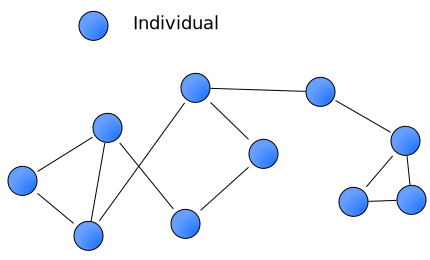
\includegraphics[width=3.2in]{social-network}
\caption{
An actor (vertice) can be an individual or organization. [3]
}
\label{fig_sim}
\end{figure}
\end{center}

\begin{center}
\begin{figure}[hb]
\centering
%\includegraphics{imagen1.eps}
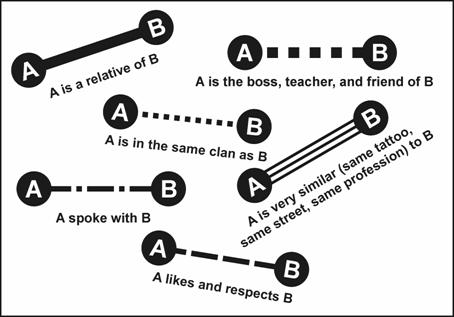
\includegraphics[width=3.2in]{f03}
\caption{
A dyad: two nodes and the edge between them. [5]
}
\label{fig_sim}
\end{figure}
\end{center}

\begin{center}
\begin{figure}[hb]
\centering
%\includegraphics{imagen1.eps}
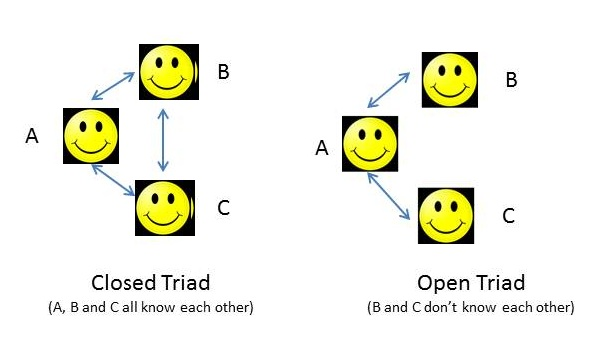
\includegraphics[width=3.2in]{open-triad}
\caption{
A triad: three nodes and the edges between them. [6]
}
\label{fig_sim}
\end{figure}
\end{center}


The three seasons used in this dataset are as per Mu (2007): 
November, December, January, February, March: 0 (winter); 
June, July, August: 1 (summer); 
April, May, September, October: 2 (shoulder) \\

\begin{center}
\begin{figure}[hb]
\centering
%\includegraphics{imagen1.eps}
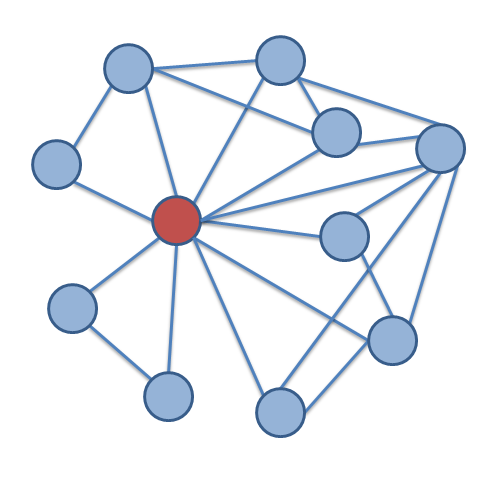
\includegraphics[width=3.2in]{ego_network}
\caption{
A node with high degree centrality. [7]
}
\label{fig_sim}
\end{figure}
\end{center}

\begin{center}
\begin{figure}[hb]
\centering
%\includegraphics{imagen1.eps}
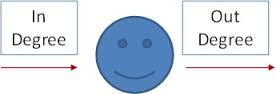
\includegraphics[width=3.2in]{degree_centrality}
\caption{
In degree and out degree in a directional social network. [8]
}
\label{fig_sim}
\end{figure}
\end{center}

\begin{center}
\begin{figure}[hb]
\centering
%\includegraphics{imagen1.eps}
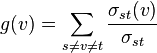
\includegraphics[width=1.5in]{betweenness_centrality}
\end{figure}
\end{center}

\begin{center}
\begin{figure}[hb]
\centering
%\includegraphics{imagen1.eps}
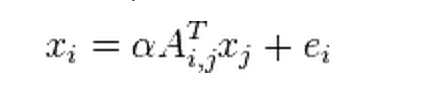
\includegraphics[width=2.0in]{alpha_centrality}
\end{figure}
\end{center}

\begin{center}
\begin{figure}[hb]
\centering
%\includegraphics{imagen1.eps}
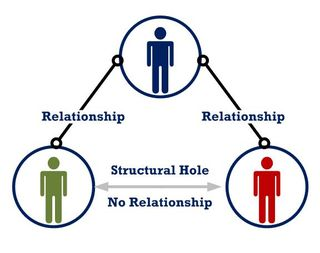
\includegraphics[width=3.2in]{structural_hole}
\caption{
A structural hole in a triad. [12]
}
\label{fig_sim}
\end{figure}
\end{center}

\section{Influence}
In preparing the dataset I first used the Google Finance feature of Google Spreadsheets to obtain end of day data for UNG
since inception (2007-04-18) until 2014-09-17\footnote{https://support.google.com/docs/answer/3093281?hl=en}. Then I processed 
the data to generate the Return, Day of Year, Season, Day of Week, Open, Overnight Change and Previous Return columns.
To calculate mean temperature I downloaded all daily weather data for the New York Central Park weather station from 1763 until 2014.
\footnote{http://www1.ncdc.noaa.gov/pub/data/ghcn/daily/by\_year/}
Originally I intended to use the observed temperature at 12:00 AM, however this data was not available for recent years.
Thus, to calculate the mean I averaged all minimum and maximum temperature measurements for a given day of the year. 
The observed temperature column I populated with the average of minimum and maximum temperature on the specific date. \\
\indent Once I had the dataset, I attempted to implement logistic regression. Unfortunately, I was not successful. I encountered
issues with float precision in Python and probably other implementation problems. I did implement a Naive Bayes classifier
successfully, however it is very slow.  In order to be able to present this report on time I resorted to developing 
a Scikit-learn based solution.[5] Thus, the rest of this section and the results discuss my findings with the aforementioned solution. \\
\indent I used leave-one-out cross-validation to test the performance of my dataset with logistic regression, LDA and Naive Bayes
classifiers, as well as to identify the best model dimension. I repeated the cross-validation experiment starting with only two
dimensions (Day of Year and Season) and adding one dimension on every run until all 8 dimensions were included in the model, for
every classifier. I also implemented a "baseline" classifier which always chooses the predominant result from the test set. \\
\indent I repeated all tests with half of the training data in order to evaluate how changing the data size affects the
performance of the classifiers. \\

\section{Viral Marketing}

% An example of a floating figure using the graphicx package.
% Note that \label must occur AFTER (or within) \caption.
% For figures, \caption should occur after the \includegraphics.

\subsection{Logistic Regression}
I first performed logistic regression with half of the dataset (923 samples):



As demonstrated in table 1, the model performs slightly better than the baseline (always choosing the most popular result). It appears that adding weather measurements (mean and
observed temperature) helps reduce both the training error rate and the estimated true prediction error.\\
\indent Next, I repeated the test with the full dataset (1847 samples), as can be seen on table 2. The results are very much consistent and show that the model of all 8
dimensions performs better than average and better than models of lower dimensions. However, my results reveal that increasing the amount of training data decreases the
performance of the model, which is unexpected. It could be explained by the fact that the dataset was not randomized. Thus, there appear to be other factors which may
help in predicting the direction of gas equities, and they could be an interesting topic for further research. \\
\indent A slight overfitting can be observed when adding the overnight return variable to the larger dataset. What is interesting
is that adding mean temperature alone does not improve performance, but adding the observed temperature does. \\

\subsection{LDA}

Table 3 summarizes the results of the LDA classifier. Similar results were obtained as with Logistic Regression. LDA performs even better on the smaller dataset,
but performs worse than Logistic Regression on the full dataset. \\


\subsection{Naive Bayes}
Table 4 shows the results of running the scikit-learn Naive Bayes classifier. The Naive Bayes classifier performs the worst of all three evaluated in this paper. A possible reason
would be that the dataset dimensions are not truly independent: season for example can be inferred from day of year. \\
I also implemented a Naive Bayes classifier, but it is much slower than the Scikit-learn version. Yet, the results are the same
(apart for some very slight differences on the smaller dataset which I attribute to including the header line in the row count and rounding). The results of my classifier
can be seen on Table 5.


While not shown, I did try various combinations of dimensions with all three classifiers and experienced similar or worse results. Therefore,
based on the results above, the model with all 8 dimensions is able to predict the direction of daily returns for natural gas securities slightly
better than the baseline, when used with Logistic Regression classifier (see fig.1) . \\

\section{Conclusion}
This is a first attempt at creating a dataset linking weather variations to intraday trading returns for a gas security. I chose the dimensions for this
dataset based primarily on empirical observations, but also validated their relevance using the leave-one-out cross-validation method. Predicting intraday
returns for any security, especially one as volatile as UNG, is a very challenging task. While the proposed dataset performs less than perfectly, it can be
used as a good starting point for further research. \\
\indent Gas supply is relatively fixed in the short term, because building wells and pipes takes time. On the other hand,
temperature fluctuations affect gas demand as consumers and industries buy more gas for heating/cooling. Thus, the changes in demand with fixed
supply lead to volatility in the equilibrium price. Traders of gas equities analyse supply and demand data to gain insight into the market direction. However,
supply, storage and demand numbers are available only on the day when a report is released. Yet, traders need to make buy/sell decisions every day the market
is open. Hence, weather appears to be the one input factor which is continuously available and affects prices. \\
Normally gas features are very volatile, still there are 36 days in the dataset
for which the intraday return is 0.00\% (open price is equal to close price). For these
days I assign the intraday return to 0 (negative).\\
\indent A possible future direction for research would be to consider temperature measurements throughout the day, as Chang et al. (2008) do for the overall market[4], but
particularly with respect to gas equities. If enough DGAZ/UGAZ data is available, it may provide better insight into the psychology of intraday traders, due to the triple
returns offered by these instruments. Other variables, such as the market demand/supply numbers, can help predict the trend for gas prices. At the same time, the
day when these numbers are reported experiences unusual returns and volatility [3]. Augmenting the daily returns prediction model with the aforementioned extra
dimensions could improve its performance, hence it would be a worthwhile direction of further research. \\

% trigger a \newpage just before the given reference
% number - used to balance the columns on the last page
% adjust value as needed - may need to be readjusted if
% the document is modified later
%\IEEEtriggeratref{8}
% The "triggered" command can be changed if desired:
%\IEEEtriggercmd{\enlargethispage{-5in}}

% references section
\begin{thebibliography}{1}
%\bibitem{Bib:King}
%M. King, B. Zhu, and S. Tang, "Optimal path planning," Mobile Robots, vol. 8, no. 2, pp. 520-531, March 2001.
%\bibitem{Bib:Simpson}
%H. Simpson, Dumb Robots, 3rd ed., Springfield: UOS Press, 2004, pp.6-9.
\bibitem{Bib:Crowdsourcing}
How to Use Crowdsourcing in the Classroom. Available: http://www.hollyclark.org/2013/11/03/how-to-use-crowdsourcing-in-the-classroom/
\bibitem{Bib:SocialNetwork}
Social Network. Available: http://en.wikipedia.org/wiki/Social\_network
\bibitem{Bib:SocialNetworkDiagram}
An example of a social network diagram. Available: http://commons.wikimedia.org/wiki/File:Social-network.png
\bibitem{Bib:Wasserman}
Wasserman, Stanley; Faust, Katherine (1994). "Social Network Analysis in the Social and Behavioral Sciences". Social Network Analysis: Methods and Applications. Cambridge University Press. pp. 1–27. ISBN 9780521387071
\bibitem{Bib:GeospatialAnalysisPrinciples}
Examples of dyads. United States Army Training Support Center. Available: https://courseware.e-education.psu.edu/courses/bootcamp/lo09/08.html
\bibitem{Bib:Tufekci}
Tufekci, Zeynep; "Is the Social Web Less Surprising? The Internet of People and Social Flâneurism," Available: http://technosociology.org/?p=693
\bibitem{Bib:Weingart}
Weingart, Scott; "Networks Demystified 2: Degree," Available: http://www.scottbot.net/HIAL/?p=6526
\bibitem{Bib:DegreeCentrality}
Keung, Tim; "Social / Organizational Network Analysis: Common Terminology (Part 3)," Available: http://hr.toolbox.com/blogs/organizational-network-mapping/social-organizational-network-analysis-common-terminology-part-3-46734
\bibitem{Bib:BetweennessCentrality}
Betweenness centrality, Available: http://en.wikipedia.org/wiki/Betweenness\_centrality
\bibitem{Bib:Bavelas}
Bavelas, Alex; "Communication patterns in task-oriented groups," J. Acoust. Soc. Am, 22
\bibitem{Bib:Austin}
Austin, David; "How Google Finds Your Needle in the Web's Haystack," Available: http://www.ams.org/samplings/feature-column/fcarc-pagerank
\bibitem{Bib:Brenegar}
Brenegar, Ed; "Connect, Communicate \& Contribute," Available: http://edbrenegar.typepad.com/leading\_questions/say-thanks-every-day/
\bibitem{Bib:Leskovec}
Jure Leskovec, Daniel Huttenlocher, and Jon Kleinberg. 2010. Predicting positive and negative links in online social networks. In Proceedings of the 19th international conference on World wide web (WWW '10). ACM, New York, NY, USA, 641-650. DOI=10.1145/1772690.1772756 http://doi.acm.org/10.1145/1772690.1772756
\bibitem{Bib:Khanafiah}
D Khanafiah , H Situngkir. Social Balance Theory. Revisiting Heider’s Balance Theory for many agents, 2004
\bibitem{Bib:Galuba}
W Galuba, S Asur, BA Huberman.Influence and passivity in social media, in Machine learning and knowledge discovery in databases, 2011, Springer Berlin Heidelberg.
\bibitem{Bib:Huberman}
BA Huberman, DM Romero, F Wu. Social networks that matter: Twitter under the microscope, inarXiv preprint arXiv:0812.1045, 2008
\bibitem{Bib:Yu}
Louis Yu, SitaramAsur and Bernardo A. Huberman. ArtificialInflation: The Real Story of Trends in SinaWeibo, in arXiv preprint arXiv:1202.0327, 2011
\bibitem{Bib:Leskovec}
Jure Leskovec, Lada A. Adamic, and Bernardo A. Huberman. 2007. The dynamics of viral marketing. ACM Trans. Web 1, 1, Article 5 (May 2007). DOI=10.1145/1232722.1232727 http://doi.acm.org/10.1145/1232722.1232727
\bibitem{Bib:Zarella}
Zarella, Dan; "Informational Cascades Prove Tipping Points Exist," Available: http://danzarrella.com/informational-cascades.html
\end{thebibliography}

\end{document}
